\documentclass[../main.tex]{subfiles}

\begin{document}

\section{Kinematics}

\subsection{Displacement}

\subsubsection*{Position}

In order to describe the motion of an object, you must first be able to describe its \gls{position}---where it is at any particular time. More precisely, you need to specify its position relative to a convenient reference frame. Earth is often used as a reference frame, and we often describe the position of an object as it relates to stationary objects in that reference frame. For example, a rocket launch would be described in terms of the position of the rocket with respect to the Earth as a whole, while a professor's position could be described in terms of where she is in relation to the nearby white board. (See Figure ?.??.) In other cases, we use reference frames that are not stationary but are in motion relative to the Earth. To describe the position of a person in an airplane, for example, we use the airplane, not the Earth, as the reference frame. (See Figure ??.?.)

\subsubsection*{Displacement}

If an object moves relative to a reference frame (for example, if a professor moves to the right relative to a white board or a passenger moves toward the rear of an airplane), then the object's position changes. This change in position is known as \gls{displacement}. The word ``displacement'' implies that an object has moved, or has been displaced.

\vspace{1ex}

\begin{mdframed}[backgroundcolor=black!10]
    \textbf{Displacement}

    \vspace{1ex}
    
    Displacement is the \textit{change in position} of an object:

    \begin{equation} \label{PhLnzc}
        \Delta{x} = x_f - x_0
    \end{equation}

    where $\Delta{x}$ is displacement, $x_f$ is final position, and $x_0$ is initial position.
\end{mdframed}

In this text the upper case Greek letter $\Delta$ (delta) always means ``change in'' whatever quantity follows it; thus, $\Delta{x}$ means \textit{change in position}. Always solve for displacement by subtracting initial position  $x_0$ from final position $x_f$.

\vspace{1em}
 .
Note that the SI unit for displacement is the meter (m) (see Physical Quantities and Units), but sometimes kilometers, miles, feet, and other units of length are used. Keep in mind that when units other than the meter are used in a problem, you may need to convert them into meters to complete the calculation.

\vspace{1em} % 2 Figures

Note that displacement has a direction as well as a magnitude. The professor's displacement is \SI{2.0}{m} to the right, and the airline passenger's displacement is \SI{4.0}{m} toward the rear. In one-dimensional motion, direction can be specified with a plus or minus sign. When you begin a problem, you should select which direction is positive (usually that will be to the right or up, but you are free to select positive as being any direction). The professor's initial position is $x_0 = \SI{1.5}{m}$ and her final position is $x_f = \SI{3.5}{m}$. Thus her displacement is

\begin{equation*}
    \Delta{x} = x_f - x_0 = \SI{3.5}{m} - \SI{1.5}{m} = +\SI{2.0}{m}
\end{equation*}

In this coordinate system, motion to the right is positive, whereas motion to the left is negative. Similarly, the airplane passenger's initial position is $x_0= \SI{6.0}{m}$ and his final position is  $x_f = \SI{2.0}{m}$, so his displacement is

\begin{equation*}
    \Delta{x} = x_f - x_0 = \SI{2.0}{m} - \SI{6.0}{m} = -\SI{4.0}{m}
\end{equation*}

His displacement is negative because his motion is toward the rear of the plane, or in the negative $x$ direction in our coordinate system.

\subsubsection*{Distance}

Although displacement is described in terms of direction, distance is not. \Gls{distance} is defined to be the magnitude or size of displacement between two positions. Note that the distance between two positions is not the same as the distance traveled between them. \Gls{distance traveled} is the total length of the path traveled between two positions. Distance has no direction and, thus, no sign. For example, the distance the professor walks is \SI{2.0}{m}. The distance the airplane passenger walks is \S{4.0}{m}.

\vspace{1ex}

\begin{mdframed}[backgroundcolor=black!10]
    \textbf{Misconception Alert: distance traveled vs.~magnitude of displacement}

    \vspace{1ex}
    
    It is important to note that the distance traveled, however, can be greater than the magnitude of the displacement (by magnitude, we mean just the size of the displacement without regard to its direction; that is, just a number with a unit). For example, the professor could pace back and forth many times, perhaps walking a distance of \SI{150}{m} during a lecture, yet still end up only \SI{2.0}{m} to the right of her starting point. In this case her displacement would be $+\SI{2.0}{m}$, the magnitude of her displacement would be \SI{2.0}{m}, but the distance she traveled would be \SI{150}{m}. In kinematics we nearly always deal with displacement and magnitude of displacement, and almost never with distance traveled. One way to think about this is to assume you marked the start of the motion and the end of the motion. The displacement is simply the difference in the position of the two marks and is independent of the path taken in traveling between the two marks. The distance traveled, however, is the total length of the path taken between the two marks.
\end{mdframed}

\begin{example} \label{bcBeYE}
    A cyclist rides \SI{3}{km} west and then turns around and rides \SI{2}{km} east. (a) What is her displacement? 
\end{example}

\Solution Although we are not given initial or final positions, we are given two separate displacements. If we define east as the positive direction, and west as the negative, as shown in the figure below, then the two displacements are

\begin{equation*}
    \Delta{x_1} = -\SI{3.0}{km} \quad \text{and} \quad \Delta{x_2} = +\SI{2.0}{km}
\end{equation*}

\begin{center}
    \begin{tikzpicture}
    \begin{axis}[width=15cm,
        axis lines = left,
        axis y line=none,
        xlabel = {Position (m)},
        ymin=0, ymax=12, 
        xmin=-4, xmax=4,
        ticks=none,
        clip=false,
        ]
        \node[right] at (4,0) {E ($+x$)};
        \node[left] at (-4,0) {W ($-x$)};
        \node[above] at (0,0) {\huge \faBicycle};
        \draw[->] (0,1) node[gray,right] {$x_0$} -- ++(axis direction cs: -3,0) node[above,pos=0.5] {$\Delta{x_1} = -\SI{3.0}{km}$};
        \draw[->] (-3,1.75) -- ++(axis direction cs: 2,0) node[above,pos=0.5] {$\Delta{x_2} = +\SI{2.0}{m}$} node[gray,right] {$x_f$};
    \end{axis}
    \end{tikzpicture}
\end{center}

The total displacement is found by summing the object's individual displacements as

\begin{equation*}
    \Delta{x} = \Delta{x_1} + \Delta{x_2} = -\SI{3.0}{km} + \SI{2.0}{km} = -\SI{1.0}{km}
\end{equation*}

The cyclist's displacement is $-\SI{1.0}{km}$, or 1.0 kilometer to the west of their original position. 

\endsolution    

\vspace{1ex}

\begin{example}
   What distance does the cyclist from Example \ref{bcBeYE} ride? 
\end{example}

\Solution To find her distance traveled, we may take the sum the \textit{magnitudes} (i.e., absolute values) of each displacement:

\begin{equation*}
    \text{distance traveled} = \lvert \Delta{x_1} \rvert + \lvert \Delta{x_2} \rvert
        = \lvert -3 \rvert + \lvert 2 \rvert 
        = 3 + 2 = 5
\end{equation*}

Therefore, her total distance traveled is \SI{5.0}{km}.

\endsolution

\vspace{1ex}

\begin{example}
    What is the magnitude of the cyclist's displacement from Example \ref{bcBeYE}?
\end{example}

\Solution In Example \ref{bcBeYE}, we calculated a displacement of $\Delta{x} = -\SI{1.0}{km}$. The magnitude of this displacement is given by the absolute value:

\begin{equation*}
    \text{magnitude of displacement} = \lvert \Delta{x} \rvert = \lvert -\SI{1.0}{km} \rvert = \SI{1.0}{km}
\end{equation*}

Since taking the absolute value is effectively dropping the negative sign, the magnitude (or size) of her displacement is 1.0 kilometer.

\endsolution

\subsection{Vectors, Scalars, and Coordinate Systems}

What is the difference between distance and displacement? Whereas displacement is defined by both direction and magnitude, distance is defined only by magnitude. Displacement is an example of a vector quantity. Distance is an example of a scalar quantity. A \gls{vector} is any quantity with both magnitude and direction. Other examples of vectors include a velocity of \SI{90}{km/h} east and a force of \SI{500}{newtons} straight down.

\vspace{1em}

The direction of a vector in one-dimensional motion is given simply by a plus ($+$) or minus ($−$) sign. Vectors are represented graphically by arrows. An arrow used to represent a vector has a length proportional to the vector's magnitude (e.g., the larger the magnitude, the longer the length of the vector) and points in the same direction as the vector.

\vspace{1em}

Some physical quantities, like distance, either have no direction or none is specified. A \gls{scalar} is any quantity that has a magnitude, but no direction. For example, a \SI{20}{\degreeCelsius} temperature, the 250 kilocalories (250 Calories) of energy in a candy bar, a \SI{90}{km/h} speed limit, a person's 1.8 m height, and a distance of 2.0 m are all scalars—quantities with no specified direction. Note, however, that a scalar can be negative, such as a  \SI{-20}{\degreeCelsius} temperature. In this case, the minus sign indicates a point on a scale rather than a direction. Scalars are never represented by arrows.

\subsubsection*{Coordinate Systems for One-Dimensional Motion}

In order to describe the direction of a vector quantity, you must designate a coordinate system within the reference frame. For one-dimensional motion, this is a simple coordinate system consisting of a one-dimensional coordinate line. In general, when describing horizontal motion, motion to the right is usually considered positive, and motion to the left is considered negative. With vertical motion, motion up is usually positive and motion down is negative. In some cases, however, as with the jet in Figure ?.?, it can be more convenient to switch the positive and negative directions. For example, if you are analyzing the motion of falling objects, it can be useful to define downwards as the positive direction. If people in a race are running to the left, it is useful to define left as the positive direction. It does not matter as long as the system is clear and consistent. Once you assign a positive direction and start solving a problem, you cannot change it.

\begin{center}
    \begin{tikzpicture}
        \begin{axis}[width=4cm,
            height=4cm,
            xmin=-1,xmax=1,
            ymin=-1,ymax=1,
            ticks=none,
            axis line style={draw=none},
            clip=false
            ]
            \draw[<->] (-1,0) node[left] {$-x$} -- (1,0) node[right] {$+x$};
            \draw[<->] (0,-1) node[below] {$-y$} -- (0,1) node[above] {$+y$};
        \end{axis}
    \end{tikzpicture}
\end{center}

\begin{example}
    A person's speed can stay the same as they round a corner and changes direction. Given this information, is speed a scalar or a vector quantity? Explain.
\end{example}

\Solution Speed is a scalar quantity. It does not change at all with direction changes; therefore, it has magnitude only. If it were a vector quantity, it would change as direction changes (even if its magnitude remained constant).

\endsolution

\subsection{Time, Velocity, and Speed}

There is more to motion than distance and displacement. Questions such as, ``How long does a foot race take?'' and ``What was the runner's speed?'' cannot be answered without an understanding of other concepts. In this section we add definitions of time, velocity, and speed to expand our description of motion.

\subsubsection*{Time}

As discussed in [Physical Quantities and Units], the most fundamental physical quantities are defined by how they are measured. This is the case with time. Every measurement of time involves measuring a change in some physical quantity. It may be a number on a digital clock, a heartbeat, or the position of the Sun in the sky. In physics, the definition of time is simple---\gls{time} is \textit{change}, or the interval over which change occurs. It is impossible to know that time has passed unless something changes.

\vspace{1em}

The amount of time or change is calibrated by comparison with a standard. The SI unit for time is the second, abbreviated s. We might, for example, observe that a certain pendulum makes one full swing every \SI{0.75}{s}. We could then use the pendulum to measure time by counting its swings or, of course, by connecting the pendulum to a clock mechanism that registers time on a dial. This allows us to not only measure the amount of time, but also to determine a sequence of events.

\vspace{1em}

How does time relate to motion? We are usually interested in elapsed time for a particular motion, such as how long it takes an airplane passenger to get from his seat to the back of the plane. To find elapsed time, we note the time at the beginning and end of the motion and subtract the two. For example, a lecture may start at 11:00 A.M. and end at 11:50 A.M., so that the elapsed time would be 50 min. \gls{elapsed time} ${\Delta}t$ is the difference between the ending time and beginning time,

\begin{equation*}
    \Delta t = t_f = t_0
\end{equation*}

where $\Delta t$ is the change in time or elapsed time, $t_f$ is the time at the end of the motion, and $t_0$ is the time at the beginning of the motion. (As usual, the delta symbol, $\Delta$, means the change in the quantity that follows it.)

\vspace{1em}

Life is simpler if the beginning time $t_0$ is taken to be zero, as when we use a stopwatch. If we were using a stopwatch, it would simply read zero at the start of the lecture and \SI{50}{min} at the end. If $t_0 = 0$, then $\Delta t = t_f \equiv t$.

\vspace{1em}

In this text, for simplicity’s sake,

\begin{itemize}
\setlength\itemsep{0.1ex}
    \item motion starts at time equal to zero ($t_0 = 0$)
    \item the symbol $t$ is used for elapsed time unless otherwise specified ($\Delta t = t_f \equiv t$)
\end{itemize}

\subsubsection*{Velocity}

Your notion of velocity is probably the same as its scientific definition. You know that if you have a large displacement in a small amount of time you have a large velocity, and that velocity has units of distance divided by time, such as miles per hour or kilometers per hour.

\begin{mdframed}[backgroundcolor=black!10]
    \Gls{average velocity} is displacement (change in position) divided by the time of travel,

    \begin{equation}
        \bar{v} = \frac{\Delta x}{\Delta t} = \frac{x_f - x_0}{t_f - t_0}
    \end{equation}

    where $\bar{v}$ is the average (indicated by the bar over the $v$) velocity, $\Delta x$ is the change in position (or displacement), and $x_f$ and $x_0$ are the final and beginning positions at times $t_f$ and $t_0$, respectively. If the starting time $t_0$ is taken to be zero, then the average velocity is simply

    \begin{equation} \label{x7GvGS}
        \bar{v} = \frac{\Delta x}{t}
    \end{equation}
\end{mdframed}

Notice that this definition indicates that velocity is a vector because displacement is a vector. It has both magnitude and direction. The SI unit for velocity is meters per second or m/s, but many other units, such as km/h, mi/h (also written as mph), and cm/s, are in common use. Suppose, for example, an airplane passenger took 5 seconds to move $-\SI{4}{m}$ (the negative sign indicates that displacement is toward the \textit{back} of the plane). His average velocity would, by Equation \eqref{x7GvGS}, be

\begin{equation*}
    \bar{v} = \frac{\Delta x}{t} = \frac{-\SI{4}{m}}{\SI{5}{s}} = -\SI{0.8}{m/s}
\end{equation*}

The minus sign indicates the average velocity is also toward the rear of the plane.

\vspace{1em}

The average velocity of an object does not tell us anything about what happens to it between the starting point and ending point, however. For example, we cannot tell from average velocity whether the airplane passenger stops momentarily or backs up before he goes to the back of the plane. To get more details, we must consider smaller segments of the trip over smaller time intervals.

\vspace{1em} %Figure

The smaller the time intervals considered in a motion, the more detailed the information. When we carry this process to its logical conclusion, we are left with an infinitesimally small interval. Over such an interval, the average velocity becomes the instantaneous velocity or the velocity at a specific instant. A car’s speedometer, for example, shows the magnitude (but not the direction) of the instantaneous velocity of the car. (Police give tickets based on instantaneous velocity, but when calculating how long it will take to get from one place to another on a road trip, you need to use average velocity.) \gls{instantaneous velocity} $v$ is the average velocity at a specific instant in time (or over an infinitesimally small time interval).

\vspace{1em}

Mathematically, finding instantaneous velocity, $v$, at a precise instant $t$ can involve taking a limit, a calculus operation beyond the scope of this text. However, under many circumstances, we can find precise values for instantaneous velocity without calculus.

\subsubsection*{Speed}

In everyday language, most people use the terms ``speed'' and ``velocity'' interchangeably. In physics, however, they do not have the same meaning and they are distinct concepts. One major difference is that speed has no direction. Thus speed is a scalar. Just as we need to distinguish between instantaneous velocity and average velocity, we also need to distinguish between instantaneous speed and average speed.

\vspace{1em}

\Gls{instantaneous speed} is the magnitude of instantaneous velocity. For example, suppose the airplane passenger at one instant had an instantaneous velocity of $−\SI{3.0}{m/s}$ (the minus meaning toward the rear of the plane). At that same time his instantaneous speed was \SI{3.0}{m/s}. Or suppose that at one time during a shopping trip your instantaneous velocity is \SI{40}{km/h} due north. Your instantaneous speed at that instant would be \SI{40}{km/h}---the same magnitude but without a direction. Average speed, however, is very different from average velocity. \gls{average speed} is the distance traveled divided by elapsed time.

\vspace{1em}

We have noted that distance traveled can be greater than the magnitude of displacement. So average speed can be greater than average velocity, which is displacement divided by time. For example, if you drive to a store and return home in half an hour, and your car’s odometer shows the total distance traveled was \SI{6}{km}, then your average speed was \SI{12}{km/h}. Your average velocity, however, was zero, because your displacement for the round trip is zero. (Displacement is change in position and, thus, is zero for a round trip.) Thus average speed is \textit{not} simply the magnitude of average velocity.

\vspace{1em} %Figure

Another way of visualizing the motion of an object is to use a graph. A plot of position or of velocity as a function of time can be very useful. For example, for this trip to the store, the position, velocity, and speed-vs.-time graphs are displayed in Figure ?.??. (Note that these graphs depict a very simplified \gls{model} of the trip. We are assuming that speed is constant during the trip, which is unrealistic given that we’ll probably stop at the store. But for simplicity’s sake, we will model it with no stops or changes in speed. We are also assuming that the route between the store and the house is a perfectly straight line.)

\begin{center}
    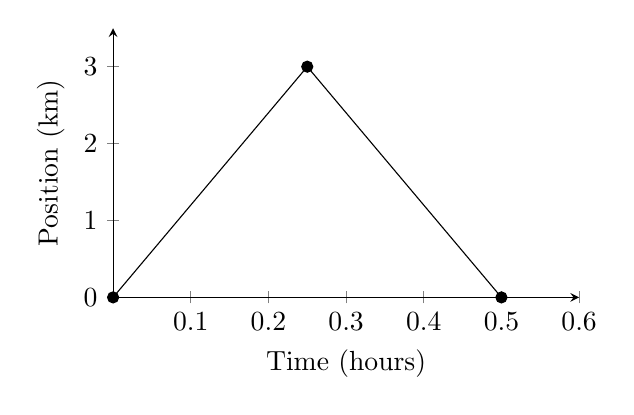
\begin{tikzpicture}
        \begin{axis}[width=7.5cm,height=5cm,
            axis lines=left,
            xmin=0,xmax=0.6,
            ymin=0,ymax=3.5,
            clip=false,
            xlabel={Time (hours)},
            ylabel={Position (km)},
            xtick={0.1,0.2,...,0.6}
        ]
        \addplot[%color=black,
            mark=*,
            ]
            coordinates {
            (0,0)(0.25,3)(0.5,0)
            };        
        \end{axis}
    \end{tikzpicture}

    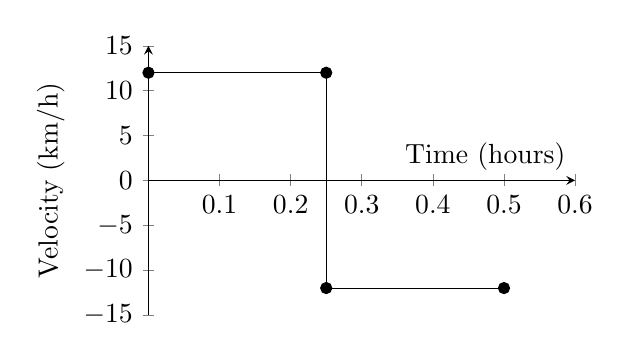
\begin{tikzpicture}
        \begin{axis}[width=7cm,height=5cm,
            axis y line=left,
            axis x line=center,
            xmin=0,xmax=0.6,
            ymin=-15,ymax=15,
            clip=false,
            ylabel={Velocity (km/h)},
            xlabel={Time (hours)},
            ytick={-15,-10,...,15},
            xtick={0.1,0.2,...,0.6}
        ]
        % \node[right=2mm] at (0.6,0) {Time (hours)};
        \addplot[%color=black,
            mark=*,
            ]
            coordinates {
            (0,12)(0.25,12)(0.25,-12)(0.5,-12)
            };
        \end{axis}
    \end{tikzpicture}

    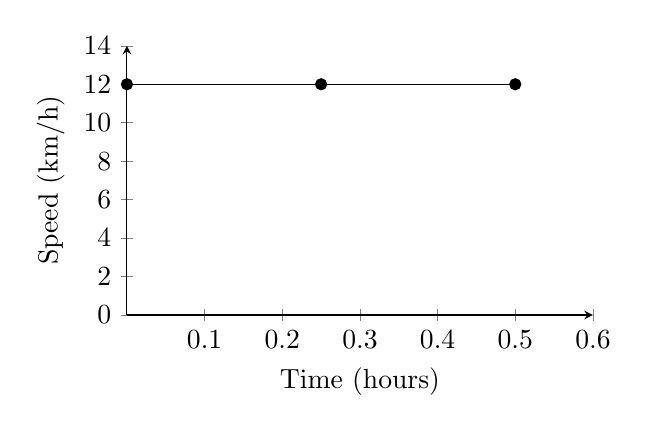
\begin{tikzpicture}
        \begin{axis}[width=7.5cm,height=5cm,
            axis lines=left,
            xmin=0,xmax=0.6,
            ymin=0,ymax=14,
            clip=false,
            xlabel={Time (hours)},
            ylabel={Speed (km/h)},
            xtick={0.1,0.2,...,0.6},
            ytick={0,2,...,14}
        ]
        \addplot[%color=black,
            mark=*,
            ]
            coordinates {
            (0,12)(0.25,12)(0.5,12)
            };        
        \end{axis}
    \end{tikzpicture}
\end{center}

\begin{mdframed}[backgroundcolor=black!10]
    If you have spent much time driving, you probably have a good sense of speeds between about 10 and 70 miles per hour. But what are these in meters per second? What do we mean when we say that something is moving at \SI{10}{m/s}? To get a better sense of what these values really mean, do some observations and calculations on your own:

    \begin{itemize}
    \setlength\itemsep{0.1ex}
        \item calculate typical car speeds in meters per second
        \item estimate jogging and walking speed by timing yourself; convert the measurements into both m/s and mi/h
        \item determine the speed of an ant, snail, or falling leaf
    \end{itemize}
\end{mdframed}

\begin{example} \label{au4Ac2}
    A commuter train travels from Baltimore to Washington, DC, and back in 1 hour and 45 minutes. The distance between the two stations is approximately 40 miles. What is the average velocity of the train?
\end{example}

\Solution The average velocity of the train is zero because $x_ f= x_0$; the train ends up at the same place it starts. 

\endsolution

\begin{example}
    What is the average speed, in meters per second, of the train from Example \ref{au4Ac2}?
\end{example}

\Solution The train travels 40 miles one way and 40 miles back, so we are given a total distance of 80 miles. Also, a time of 1 hour and 45 minutes is equivalent to 105 minutes. Average speed is given by

\begin{equation*}
    \text{average speed} = \frac{\text{distance}}{\text{time}} = \frac{\text{80 miles}}{\text{105 minutes}}
\end{equation*}

We convert miles per minutes to meters per second using dimensional analysis as follows:

\begin{equation*}
    \frac{\text{80 miles}}{\text{105 minutes}}
    \times \frac{\text{5280 feet}}{\text{1 mile}}
    \times \frac{\text{1 meter}}{\text{3.28 feet}}
    \times \frac{\text{1 minute}}{\text{60 seconds}} = \SI{20}{m/s}
\end{equation*}



\end{document}